\section{TODO}

commands format stick:

lsblk to find mounted devices
unmount device:  sudo umount /dev/sdc1

hier RICHTIG SCHÖN ZEIT LASSEN, IMMER NEUE ZEILE MIT KÄSTCHEN!!!!!

 sudo mkfs -t ext3 /dev/sdc

allo \cite{Sciencedirect.07.01.2022}  welt

\begin{figure}[H]
	\centering
	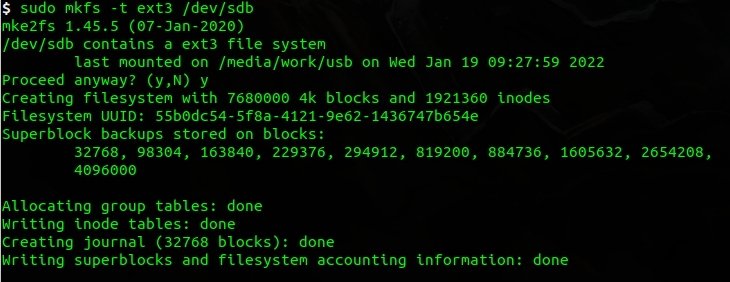
\includegraphics[width=12cm,keepaspectratio=true]{pictures/createfs.png}
	\caption{
		Erstellen eines EXT3 Dateisystems auf einem USB Stick
	}
	\label{fig:createfs}
\end{figure}

TODO: GENAU BESCHREIBEN WAS DA PASSIERT!

\section{Introduction and history}

Das sogenannte \ac{ext} war das erste einer Reihe von Dateisystemen welches speziell für Linux entwickelt wurde und damals das minix Dateisystem ablöste. EXT in Version 1 ist mittlerweile allerdings veraltet und wird in aktuellen Linuxdistributionen nicht mehr verwendet. Die folgenden Erweiterungen existieren:

\begin{itemize}
	\item ext2 - Führte separate Zeitstempel für Dateizugriffe, inode- und Datenmodifikation. Bringt keine Unterstützung für journaling.
	\item ext3 - Führt journaling ein (und ist required!)
	\item ext4 - Unterstützung für fast fsck[1], native filesystem encryption[2], journaling, jedoch auch für non-journaling.
\end{itemize}

% TODO
- Journaling beschreiben!
- Intro to EXT allgemein, siehe Fragen in der Aufgabenstellung


